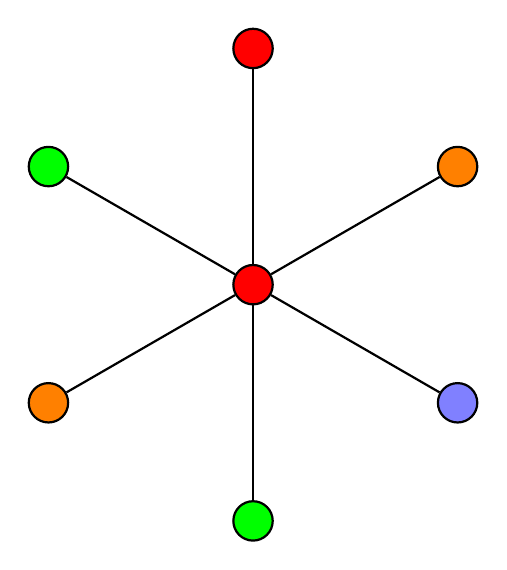
\begin{tikzpicture}[
	% Define the style for the nodes
	every node/.style={circle, draw, thick, minimum size=5mm}
	]
	
	% --- VERTICES ---
	% Format: \node (internal_name) at (x,y) [fill=color] {number};
	
	\node (v1) at (0, 0) [fill=red]  {};
	\node (v2) at (0, 3) [fill=red] {};
	\node (v3) at (2.598, 1.5) [fill=orange]{};
	\node (v4) at (-2.598, 1.5) [fill=green]{};
	\node (v5) at (2.598, -1.5) [fill=blue!50]{};
	\node (v6) at (-2.598, -1.5) [fill=orange]{};
	\node (v7) at (0, -3) [fill=green]{};
	
	% --- EDGES ---
	% In a K4, there are 6 possible edges. 
	% We omit one (e.g., the diagonal between v1 and v4).
	
	\draw[thick] (v1) -- (v2);
	\draw[thick] (v1) -- (v3);
	\draw[thick] (v1) -- (v4);
	\draw[thick] (v1) -- (v5);
	\draw[thick] (v1) -- (v6);
	\draw[thick] (v1) -- (v7);
	
\end{tikzpicture}